\documentclass[aspectratio=169,11pt]{beamer}

\usetheme{Madrid}
\usecolortheme{default}
\usefonttheme{professionalfonts}

\usepackage[utf8]{inputenc}
\usepackage[T1]{fontenc}
\usepackage{lmodern}
\usepackage{graphicx}
\usepackage{multicol}
\usepackage{booktabs}
\usepackage{array}
\usepackage{tikz}
\usepackage{tikz-cd}
\usepackage{pgfplots}
\usepackage{smartdiagram}
\usepackage{listings}
\usepackage{animate}
\usepackage{xcolor}
\usepackage{hyperref}
\usepackage{ragged2e}
\usepackage{ifthen}
\usepackage{tabularx}
\usepackage{fontawesome}
\providecommand{\faMicrochip}{\faCogs}
\providecommand{\faServer}{\faDatabase}
\providecommand{\faCode}{\faLaptop}
\providecommand{\faMap}{\faGlobe}
\providecommand{\faBarChart}{\faSignal}
\providecommand{\faMobile}{\faPhone}
\usetikzlibrary{arrows.meta,positioning,shapes.geometric,shapes.misc,shapes.symbols,calc,fit,backgrounds,decorations.pathmorphing,shadows.blur,matrix}
\pgfplotsset{compat=1.18}

% ---------- Color palette ----------
\definecolor{JRBlue}{HTML}{073B7A}
\definecolor{JRDeep}{HTML}{031A35}
\definecolor{JRCyan}{HTML}{00D4FF}
\definecolor{JRAqua}{HTML}{1EE3CF}
\definecolor{JRSoft}{HTML}{EAF8FF}
\definecolor{JRWarn}{HTML}{FFB703}
\definecolor{JRDanger}{HTML}{E63946}
\definecolor{JRHigh}{HTML}{F77F00}
\definecolor{JRMed}{HTML}{F4D35E}
\definecolor{JRLow}{HTML}{2A9D8F}
\definecolor{JRGray}{HTML}{5A6473}

\setbeamercolor{palette primary}{bg=JRBlue,fg=white}
\setbeamercolor{palette secondary}{bg=JRCyan,fg=JRDeep}
\setbeamercolor{palette tertiary}{bg=JRDeep,fg=white}
\setbeamercolor{frametitle}{bg=JRBlue,fg=white}
\setbeamercolor{title}{fg=white,bg=JRBlue}
\setbeamercolor{block title}{bg=JRBlue,fg=white}
\setbeamercolor{block body}{bg=JRSoft,fg=JRDeep}
\setbeamercolor{normal text}{fg=JRDeep,bg=white}
\setbeamertemplate{navigation symbols}{}
\setbeamertemplate{footline}{\leavevmode\hbox to \paperwidth{\hfill\color{JRGray}\scriptsize JalRakshak v2 \quad \insertframenumber/\inserttotalframenumber\hspace{0.3cm}}\vspace{0.15cm}}
\setbeamertemplate{section in toc}[circle]

% ---------- Helpers ----------
\newcommand{\chip}[2]{\tikz[baseline=(X.base)]\node[rounded corners=2pt,fill=#1!15,draw=#1,text=#1,inner xsep=5pt,inner ysep=2pt,font=\scriptsize\bfseries](X){#2};}
\newcommand{\metric}[3]{\begin{tikzpicture}\node[rounded corners=5pt,fill=#1!12,draw=#1,thick,minimum width=2.25cm,minimum height=1.15cm,align=center]{\Large\bfseries #2\\[-1pt]\scriptsize #3};\end{tikzpicture}}
\newcommand{\placeholderimage}[3]{\IfFileExists{#1}{\includegraphics[width=#2,height=#3,keepaspectratio]{#1}}{\begin{tikzpicture}\node[draw=JRCyan,dashed,rounded corners=6pt,fill=JRSoft,minimum width=#2,minimum height=#3,align=center,text=JRGray]{Place image file:\\ \texttt{\detokenize{#1}}};\end{tikzpicture}}}
\newcommand{\zonecard}[4]{\begin{tikzpicture}\node[rounded corners=7pt,fill=#4!13,draw=#4,thick,minimum width=2.45cm,minimum height=1.45cm,align=left,inner sep=4pt]{\textbf{#1}\\\scriptsize pH: #2 \quad Turbidity: #3\\\chip{#4}{RISK: #1}};\end{tikzpicture}}
\tikzset{box/.style={rounded corners=5pt,draw=JRBlue,thick,fill=JRSoft,align=center,minimum height=0.8cm,drop shadow}, process/.style={box,fill=JRCyan!12}, data/.style={cylinder,shape border rotate=90,aspect=0.25,draw=JRBlue,fill=JRAqua!12,align=center,minimum height=0.9cm}, arrow/.style={-{Latex[length=2.5mm]},thick,draw=JRBlue}}

\title[JalRakshak v2]{\Huge JalRakshak v2}
\subtitle{\textcolor{white}{AI-Powered Post-Flood Water Quality Monitoring \& Disease Outbreak Prediction}}
\date{\textcolor{white}{Built for Assam. Built for every flood-prone district in India.}}

\begin{document}

% 1
{\usebackgroundtemplate{
\begin{tikzpicture}[remember picture,overlay]\shade[left color=JRDeep,right color=JRBlue] (current page.south west) rectangle (current page.north east);\node[opacity=.10,text=white,scale=9] at (current page.center){JalRakshak};\foreach \x in {0,1,...,15}{\draw[JRCyan!25] (\x,0) -- +(2,9);}\end{tikzpicture}}
\begin{frame}[plain]\vspace{0.45cm}\titlepage\vfill\centering\chip{JRCyan}{AI} \chip{JRAqua}{IoT} \chip{JRWarn}{Disaster Response} \chip{JRLow}{PWA Offline}\end{frame}}

\section{Problem \& Opportunity}
% 2
\begin{frame}{Problem Statement: Floods Trigger a Second Crisis}
\Large\textbf{Assam floods kill people twice: first the water, then disease.}\normalsize
\begin{itemize}
\item Cholera, typhoid, hepatitis A and leptospirosis rise after floodwater contaminates wells and community sources.
\item Communities lack real-time water safety intelligence and depend on delayed field sampling.
\item Without early warning, contamination becomes a preventable public-health emergency.
\end{itemize}
\vspace{0.15cm}
\centering
\metric{JRDanger}{5M+}{displaced annually}\hspace{0.15cm}
\metric{JRHigh}{40\%}{deaths linked to disease}\hspace{0.15cm}
\metric{JRWarn}{72h}{detection delay}\hspace{0.15cm}
\metric{JRBlue}{0}{real-time systems}\vspace{0.25cm}

\begin{tikzpicture}\node[rounded corners=8pt,fill=JRDanger!10,draw=JRDanger,thick,align=center,minimum width=8.5cm,minimum height=0.8cm]{\faWarning\ \textbf{No data, no prediction, no prevention}};\end{tikzpicture}
\end{frame}

% 3
\begin{frame}{Existing System Problems}
\begin{columns}[T]
\column{0.42\textwidth}\begin{itemize}\item Manual reporting and field visits\item WhatsApp-based updates\item Delayed response and fragmented records\item No predictive analytics\item Limited multilingual support\item Internet failure during floods\end{itemize}
\column{0.58\textwidth}\small\begin{tabularx}{\linewidth}{>{\bfseries}p{2.8cm}XX}\toprule
Capability & Traditional System & JalRakshak \\\midrule
Detection & Delayed lab checks & Live pH, turbidity, TDS, temp \\
Prediction & Reactive & AI risk levels with confidence \\
Communication & Manual calls/messages & SMS, dashboard, chatbot \\
Access & Internet dependent & Offline-first PWA cache \\
Language & Mostly English/Hindi & English, Hindi, Assamese \\
\bottomrule\end{tabularx}
\end{columns}
\end{frame}

\section{Solution}
% 4
\begin{frame}{JalRakshak: End-to-End Flood Water Intelligence}
\centering
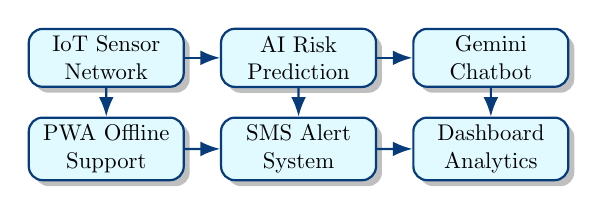
\begin{tikzpicture}[node distance=0.45cm and 0.55cm,scale=.82,transform shape]
\node[process,minimum width=2.4cm] (iot) {IoT Sensor\\Network};
\node[process,right=of iot,minimum width=2.4cm] (ai) {AI Risk\\Prediction};
\node[process,right=of ai,minimum width=2.4cm] (chat) {Gemini\\Chatbot};
\node[process,below=of iot,minimum width=2.4cm] (pwa) {PWA Offline\\Support};
\node[process,right=of pwa,minimum width=2.4cm] (sms) {SMS Alert\\System};
\node[process,right=of sms,minimum width=2.4cm] (dash) {Dashboard\\Analytics};
\foreach \src/\dst in {iot/ai,ai/chat,pwa/sms,sms/dash,iot/pwa,ai/sms,chat/dash}{\draw[arrow] (\src)--(\dst);}
\end{tikzpicture}
\vspace{0.35cm}
\begin{block}{Core Idea}\centering Transform raw floodwater readings into actionable disease-risk intelligence for citizens and health officials.\end{block}
\end{frame}

%5
\begin{frame}{Hardware Overview: Flood Water Sensing Prototype}
\begin{columns}[T]
\column{0.56\textwidth}
\resizebox{\linewidth}{!}{%
\begin{tikzpicture}[node distance=0.55cm and 0.55cm,scale=.78,transform shape]
\node[box] (ph) {pH Sensor};\node[box,below=of ph] (tur) {Turbidity Sensor};\node[box,below=of tur] (tds) {TDS Sensor};\node[box,below=of tds] (temp) {Temperature Sensor};
\node[process,right=1.8cm of tur,minimum width=2.7cm,minimum height=2.5cm] (arduino) {\faMicrochip\\\textbf{Arduino UNO}\\ADC + calibration};
\node[box,right=1.8cm of arduino] (lcd) {LCD Display\\16x2 status};\node[process,below=0.7cm of lcd] (cloud) {Future Cloud\\API / MQTT};
\foreach \sensor in {ph,tur,tds,temp}{\draw[arrow] (\sensor.east) -- (arduino.west);} \draw[arrow] (arduino) -- (lcd); \draw[arrow] (arduino.south east) -- (cloud.west);
\node[box,fit=(ph)(temp),label=above:\textbf{Water Probe Array},inner sep=8pt]{};
\begin{minipage}{0.35\textwidth}
       \hspace*{-47pt}\raisebox{-122.5pt}{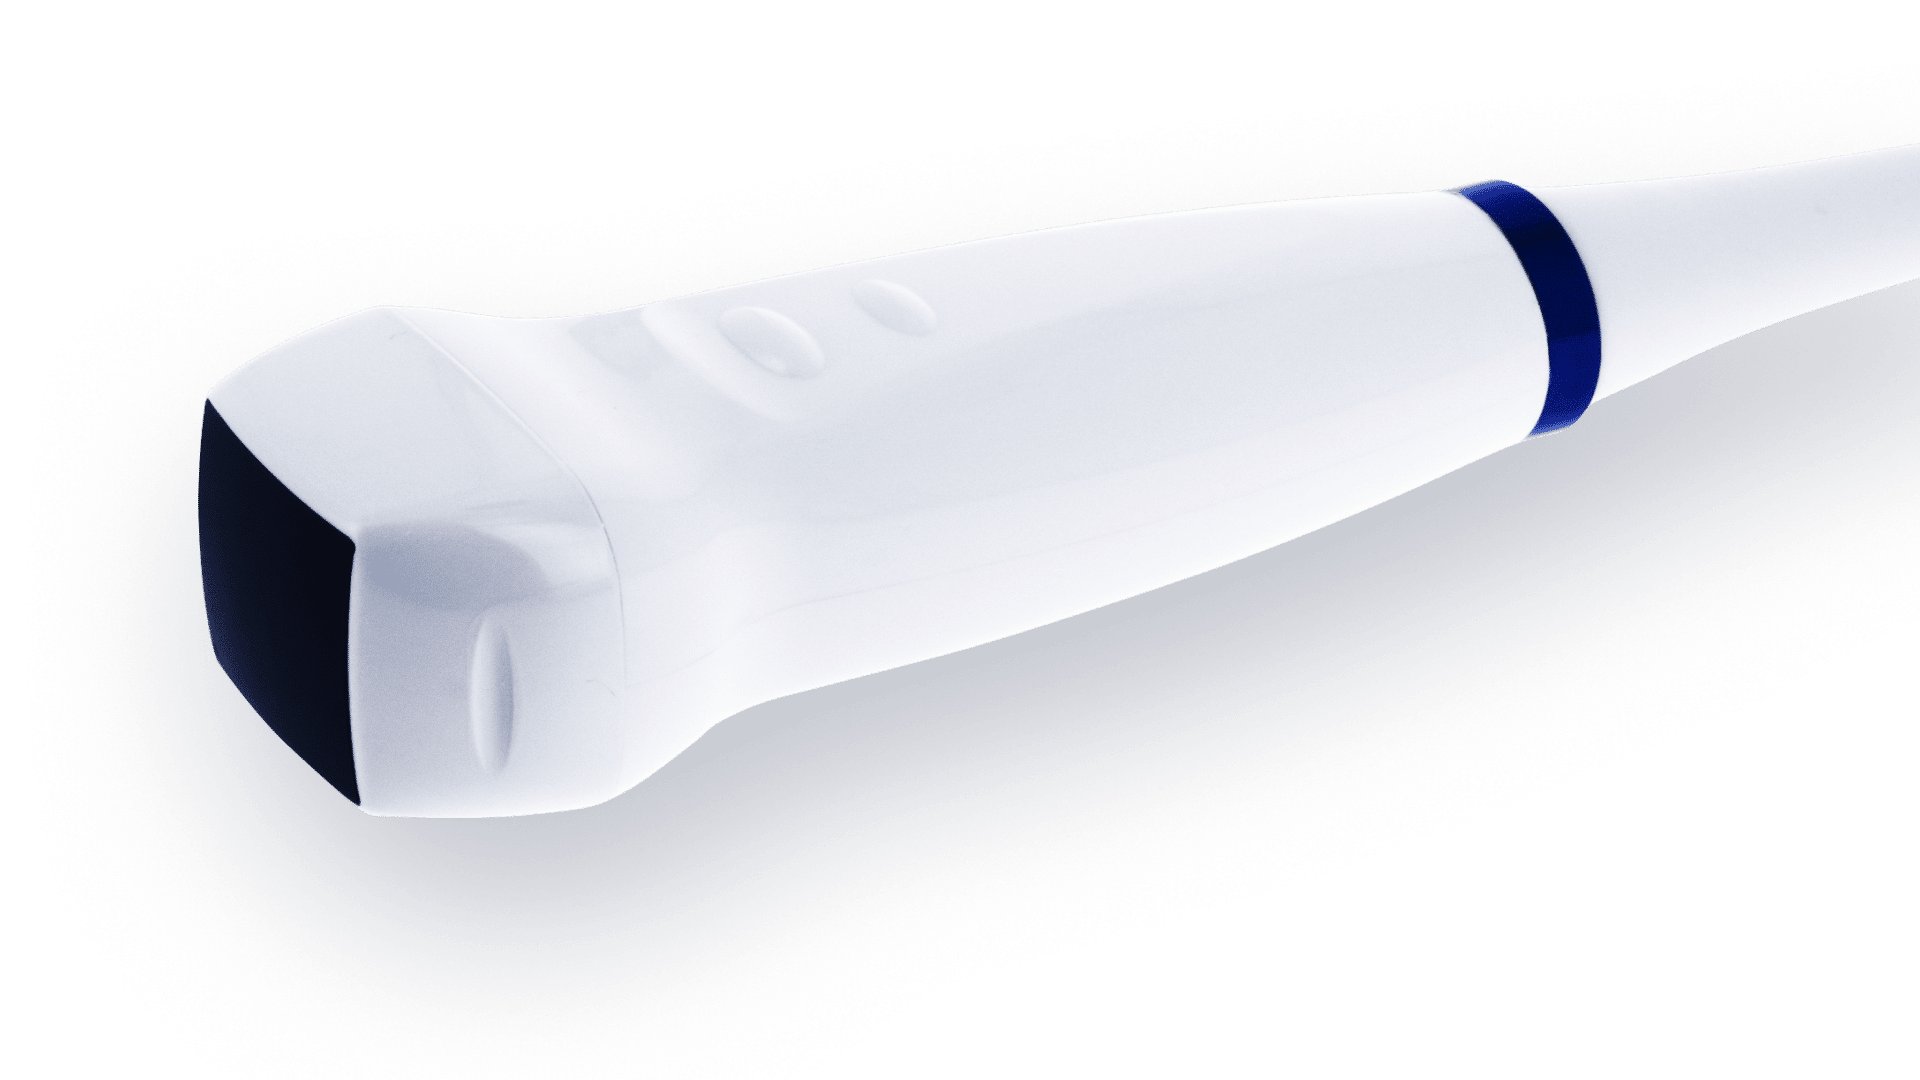
\includegraphics[width=\linewidth]{111.png}}
    \end{minipage}%  

\end{tikzpicture}}
\scriptsize\begin{itemize}\item Sensors collect pH, turbidity, dissolved solids and temperature.\item Arduino processes analog values using calibration constants.\item LCD shows real-time prototype readings.\item Breadboard, resistors and potentiometer stabilize sensor/LCD circuits.\end{itemize}
\column{0.44\textwidth}\centering\placeholderimage{images/hardware_setup.png}{6cm}{2.8cm}\vspace{0.50cm}
\begin{block}{Prototype Note}\scriptsize This prototype continuously monitors water quality parameters during floods.\end{block}
\end{columns}
\end{frame}

%6
\begin{frame}{Working Principle}
\centering\resizebox{0.93\textwidth}{!}{%
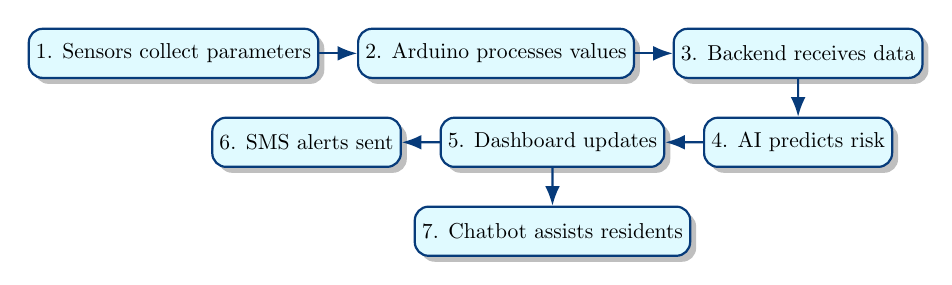
\begin{tikzpicture}[node distance=0.62cm,scale=.78,transform shape]
\node[process] (s1) {1. Sensors collect parameters};\node[process,right=of s1] (s2) {2. Arduino processes values};\node[process,right=of s2] (s3) {3. Backend receives data};
\node[process,below=of s3] (s4) {4. AI predicts risk};\node[process,left=of s4] (s5) {5. Dashboard updates};\node[process,left=of s5] (s6) {6. SMS alerts sent};\node[process,below=of s5] (s7) {7. Chatbot assists residents};
\foreach \from/\to in {s1/s2,s2/s3,s3/s4,s4/s5,s5/s6,s5/s7}{\draw[arrow] (\from)--(\to);} 
\end{tikzpicture}}\vspace{0.25cm}\hspace{0.50cm}
\scriptsize\chip{JRCyan}{Transition-ready workflow for presentation mode}
\end{frame}

%7
\begin{frame}{System Architecture}
\centering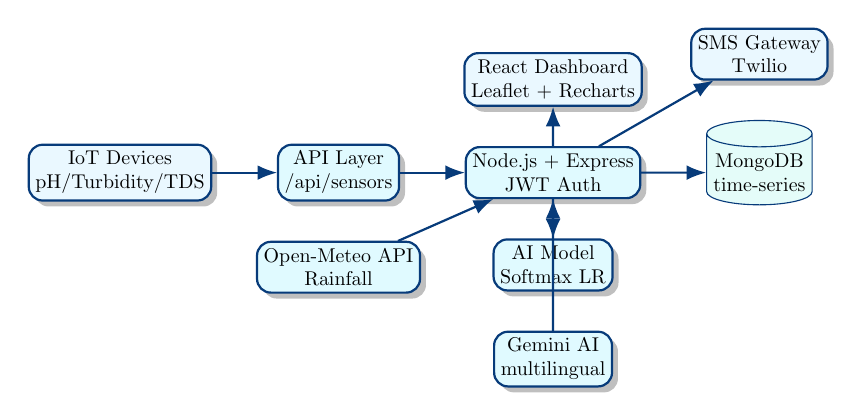
\begin{tikzpicture}[node distance=0.7cm and 1.15cm,scale=.72,transform shape]
\node[box] (iot) {IoT Devices\\pH/Turbidity/TDS};\node[process,right=of iot] (api) {API Layer\\/api/sensors};\node[process,right=of api] (node) {Node.js + Express\\JWT Auth};\node[data,right=of node] (mongo) {MongoDB\\time-series};
\node[process,below=of node] (ai) {AI Model\\Softmax LR};\node[process,below=of api] (weather) {Open-Meteo API\\Rainfall};\node[process,below=of ai] (gemini) {Gemini AI\\multilingual};
\node[box,above=of node] (dash) {React Dashboard\\Leaflet + Recharts};\node[box,above=of mongo] (sms) {SMS Gateway\\Twilio};
\draw[arrow] (iot)--(api);\draw[arrow] (api)--(node);\draw[arrow] (node)--(mongo);\draw[arrow] (node)--(ai);\draw[arrow] (weather)--(node);\draw[arrow] (gemini)--(node);\draw[arrow] (node)--(dash);\draw[arrow] (node)--(sms);
\end{tikzpicture}
\end{frame}

\section{AI, IoT \& Product}
%8
\begin{frame}{AI / Machine Learning Model}
\begin{columns}[T]\column{0.48\textwidth}\small
\begin{itemize}\item Multinomial logistic regression with softmax classification.\item 12,480 CPCB-based Brahmaputra Basin water samples.\item Features: pH deviation, turbidity norm, contamination norm, rainfall norm, contamination $\times$ rainfall.\item Outputs: \chip{JRLow}{LOW} \chip{JRMed}{MEDIUM} \chip{JRHigh}{HIGH} \chip{JRDanger}{CRITICAL}\end{itemize}
\column{0.52\textwidth}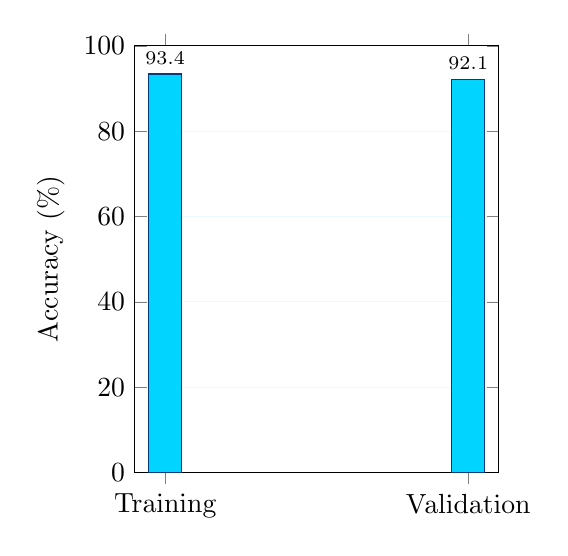
\begin{tikzpicture}\begin{axis}[ybar,bar width=12pt,width=6.2cm,height=7.0cm,ymin=0,ymax=100, ylabel={Accuracy (\%)}, symbolic x coords={Training,Validation},xtick=data,nodes near coords, nodes near coords align={vertical},every node near coord/.append style={font=\scriptsize},major grid style={draw=JRSoft},ymajorgrids=true]
\addplot[fill=JRCyan,draw=JRBlue] coordinates {(Training,93.4) (Validation,92.1)};\end{axis}\end{tikzpicture}\end{columns}
\end{frame}

%9
\begin{frame}{IoT \& Real-Time Monitoring}
\begin{columns}[T]\column{0.50\textwidth}\small\begin{itemize}\item pH monitoring detects acidic/alkaline deviations.\item Turbidity and TDS indicate suspended solids and contamination risk.\item Rainfall from Open-Meteo improves outbreak context.\item Device metadata tracks GPS, signal strength, battery and calibration time.\end{itemize}
\column{0.50\textwidth}\centering\resizebox{\linewidth}{!}{%
\begin{tabular}{cc}
\zonecard{Zone A}{5.8}{72 NTU}{JRDanger} & \zonecard{Zone B}{6.1}{58 NTU}{JRHigh}\\[0.30cm]
\zonecard{Zone C}{6.4}{44 NTU}{JRMed} & \zonecard{Zone D}{7.1}{18 NTU}{JRLow}
\end{tabular}}\end{columns}
\end{frame}

%10
\begin{frame}{Dashboard \& Analytics}
\begin{columns}[T]\column{0.55\textwidth}\begin{itemize}\item Live zone dashboard with map visualization.\item MongoDB time-series storage with 7-day TTL.\item 24-hour pH, turbidity and contamination trends.\item Auto-refresh every 30 seconds with SSE alerts.\end{itemize}
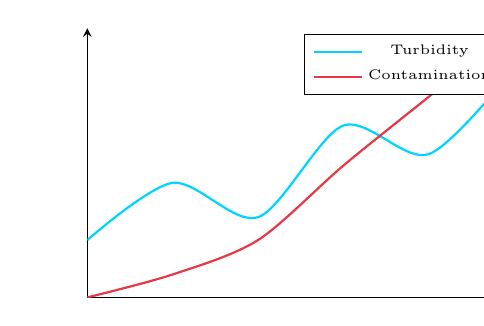
\begin{tikzpicture}\hspace{.75cm}\begin{axis} [width=7cm,height=5cm,axis lines=left,xtick=\empty,ytick=\empty,smooth,legend style={font=\tiny}]\addplot[JRCyan,thick] coordinates{(0,3)(1,4)(2,3.4)(3,5)(4,4.5)(5,6)};\addlegendentry{Turbidity}\addplot[JRDanger,thick] coordinates{(0,2)(1,2.4)(2,3)(3,4.3)(4,5.5)(5,6.7)};\addlegendentry{Contamination}\end{axis}\end{tikzpicture}
\column{0.45\textwidth}\centering\placeholderimage{images/dashboard.jpeg}{5.6cm}{5.6cm}\end{columns}
\end{frame}

%11
\begin{frame}{AI Chatbot: Gemini-Powered Resident Assistant}
\begin{columns}[T]\column{0.46\textwidth}\begin{itemize}\item Multilingual support: English, Hindi and Assamese.\item Auto-detects language and replies in the same language.\item Injects live sensor context by zone.\item Provides safety guidance and emergency next steps.\end{itemize}
\column{0.54\textwidth}\scriptsize
\setlength{\fboxsep}{5pt}
\colorbox{JRSoft}{\begin{minipage}{0.94\linewidth}
\textbf{Sample Conversation}\par\vspace{3pt}
\textbf{Resident:} Can I drink water in Zone A?\par\vspace{3pt}
\textbf{JalRakshak:} Zone A is CRITICAL: pH 5.8, contamination 81\%. Boil water or use bottled water until contamination drops below the safe threshold.\par\vspace{3pt}
\textbf{Hindi:} Paani kab safe hoga?\par\vspace{3pt}
\textbf{AI:} Jab risk LOW ho aur official alerts clear ho jayein.
\end{minipage}}\end{columns}
\end{frame}

%12
\begin{frame}{Offline-First PWA}
\begin{columns}[T]\column{0.46\textwidth}\begin{itemize}\item Floods destroy connectivity when alerts matter most.\item Service workers cache app shell, map tiles, sensor snapshots and alerts.\item Network-first data with graceful fallback to last known readings.\item Offline banner keeps users informed.\end{itemize}
\column{0.54\textwidth}\centering\resizebox{\linewidth}{!}{%
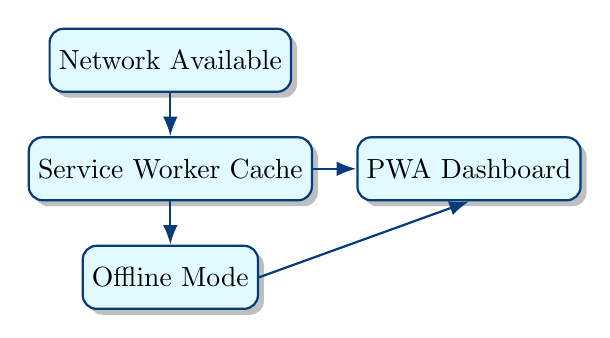
\begin{tikzpicture}[node distance=.55cm]\node[process] (net){Network Available};\node[process,below=of net] (cache){Service Worker Cache};\node[process,below=of cache] (offline){Offline Mode};\node[process,right=of cache] (ui){PWA Dashboard};\draw[arrow](net)--(cache);\draw[arrow](cache)--(offline);\draw[arrow](cache)--(ui);\draw[arrow](offline.east)--(ui.south);\end{tikzpicture}}\end{columns}
\end{frame}

%13
\begin{frame}{Emergency Response Features}
\begin{multicols}{2}\begin{itemize}\item SOS requests with location and status.\item Supply requests for water, food and medicines.\item Alert broadcasting by verified health officials.\item Emergency communication during blackouts.\item Public read-only access with official escalation.\item PDF reports for field teams and administrators.\end{itemize}\end{multicols}
\centering\begin{tikzpicture}\hspace{0.75}\node[starburst,draw=JRDanger,fill=JRDanger!15,minimum width=2.6cm,align=center]{\faAmbulance\\SOS};\node[box,right=0.65cm] {Relief Camps And Health Officials};\end{tikzpicture}
\end{frame}

%14
\begin{frame}{Tech Stack}
\centering\resizebox{0.92\textwidth}{!}{%
\begin{tikzpicture}[node distance=.35cm and .45cm]\foreach \name/\icon/\xx/\yy in {React/\faCode/0/0,Node.js/\faDatabase/1/0,Express/\faServer/2/0,Arduino/\faMicrochip/2/-2,Twilio/\faPhone/1/-2,Leaflet/\faMap/3/0,Recharts/\faBarChart/0/-2,Open-Meteo/\faBolt/3/-2}{\node[rounded corners=6pt,fill=JRSoft,draw=JRCyan,minimum width=2.7cm,minimum height=.9cm,align=center] at (\xx*3,\yy*1.05) {\icon\\\scriptsize\textbf{\name}};}\end{tikzpicture}}
\end{frame}

%15
\begin{frame}{Impact}
\begin{columns}[T]\column{0.55\textwidth}\begin{itemize}\item Faster outbreak detection and response.\item Reduced waterborne disease spread.\item Multilingual accessibility for local communities.\item Scalable deployment for flood-prone districts.\item Stronger disaster resilience and governance.\end{itemize}
\column{0.45\textwidth}\centering\resizebox{0.78\linewidth}{!}{%
\begin{tabular}{cc}
\placeholderimage{images/sdg.png}{11cm}{11cm} & 
\end{tabular}}\end{columns}
\end{frame}

\section{Roadmap \& Demo}
%16
\begin{frame}{Future Scope: Roadmap}
\centering\resizebox{0.94\textwidth}{!}{%
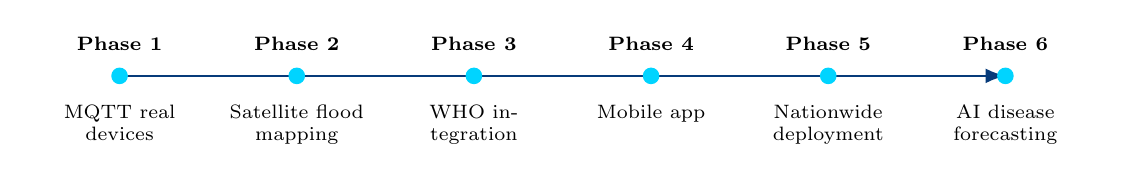
\begin{tikzpicture}[x=2.25cm,y=1cm]\draw[arrow] (0,0)--(5,0);\foreach \xx/\phase/\desc in {0/Phase 1/MQTT real devices,1/Phase 2/Satellite flood mapping,2/Phase 3/WHO integration,3/Phase 4/Mobile app,4/Phase 5/Nationwide deployment,5/Phase 6/AI disease forecasting}{\fill[JRCyan] (\xx,0) circle (3pt);\node[above=.2cm,align=center,font=\scriptsize\bfseries] at (\xx,0){\phase};\node[below=.25cm,align=center,font=\scriptsize,text width=2.1cm] at (\xx,0){\desc};}\end{tikzpicture}}
\end{frame}

%17
\begin{frame}{Challenges Faced}
\begin{columns}\column{0.5\textwidth}\begin{itemize}\item Sensor calibration across changing floodwater conditions.\item Network instability in submerged or remote areas.\item Data reliability and missing-value handling.\end{itemize}\column{0.5\textwidth}\begin{itemize}\item Multilingual AI prompt design and safety.\item Offline synchronization after reconnection.\item Balancing low-cost hardware with trustworthy readings.\end{itemize}\end{columns}
\end{frame}

%18
\begin{frame}{Demo / Prototype}
\centering\placeholderimage{images/Location.jpeg}{4.4cm}{2.7cm}\hspace{0.15cm}\placeholderimage{images/hardware_setup.png}{4.4cm}{2.7cm}\hspace{0.15cm}\placeholderimage{images/chatbot.jpeg}{4.4cm}{2.7cm}\vspace{0.35cm}
\begin{block}{Demo Flow}\centering Sensor reading $\rightarrow$ AI prediction $\rightarrow$ dashboard alert $\rightarrow$ SMS/chatbot guidance.\end{block}
\end{frame}

\begin{frame}{Prototype}
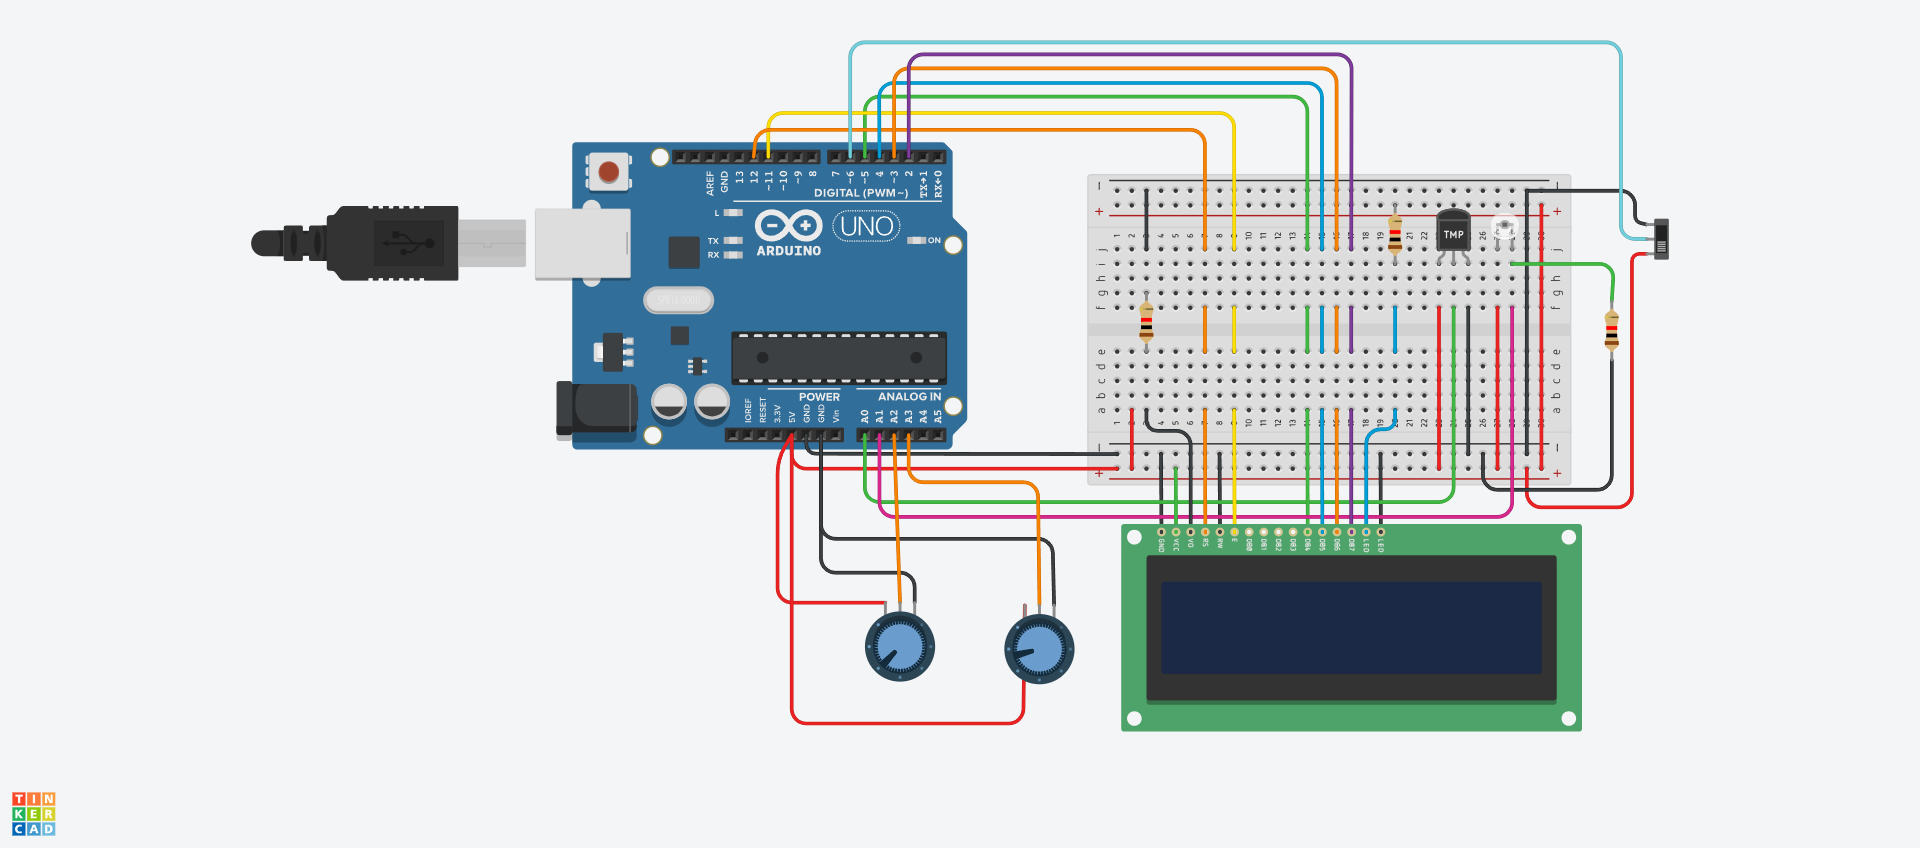
\includegraphics[width=15cm]{images/hardware_setup.png}
\end{frame}

%19
\begin{frame}{Conclusion}
\Large\textbf{JalRakshak combines AI + IoT + Disaster Management to protect flood-prone communities.}\normalsize\vspace{0.35cm}
\begin{itemize}\item Converts water quality signals into real-time safety intelligence.\item Helps citizens avoid unsafe water before outbreaks spread.\item Gives officials a dashboard, alerts and reports for faster action.\end{itemize}
\centering\vspace{0.3cm}
\begin{tikzpicture}\node[rounded corners=8pt,fill=JRBlue,text=white,minimum width=11cm,minimum height=1cm]{\Large From flood response to flood resilience.};\end{tikzpicture}
\end{frame}

%20
\begin{frame}[plain]
\begin{tikzpicture}[remember picture,overlay]\shade[left color=JRDeep,right color=JRBlue] (current page.south west) rectangle (current page.north east);\draw[JRCyan!35,line width=1.5pt] ($(current page.center)+(-5,-1.7)$)--($(current page.center)+(5,-1.7)$);\end{tikzpicture}
\centering\color{white}\vspace{1.4cm}{\Huge\bfseries Thank You}\\[0.4cm]{\LARGE Questions?}\\[0.4cm]\chip{JRCyan}{Real ML} \chip{JRAqua}{IoT Prototype} \chip{JRWarn}{PWA Offline} \chip{JRLow}{AI Chatbot}
\end{frame}

\end{document}
